\subsection*{Библиотека C++ [4]}
\begin{center}
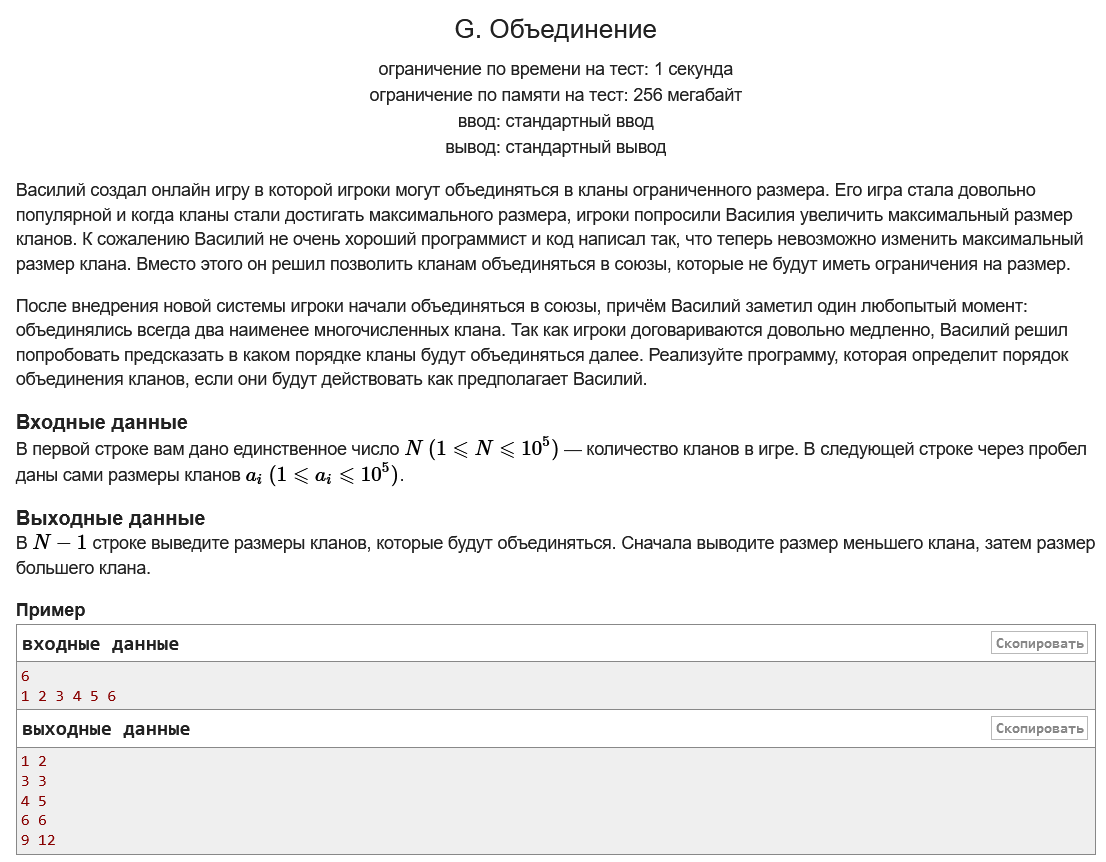
\includegraphics[width=\textwidth]{6G.png}
\end{center}
\subsubsection*{Идея решения}
Будем имитировать численность каждого клана в отсортированном состоянии благодаря типу multiset. Далее заведем цикл с $n-1$ итераций, где будем брать два минимальных элемента, выводить их и класть сумму в multiset. 
\subsubsection*{Исходный код}
\begin{lstlisting}
#include <iostream>
#include <string>
#include <unordered_map>
#include <unordered_set>
#include <map>
#include <set>
#include <algorithm>
#include <vector>
#include <cmath>
#include <iomanip>
using namespace std;
typedef long long ll;


int main()
{
    ios_base::sync_with_stdio(false);
    cin.tie(0);
    cout.tie(0);
    ll n;
    cin >> n;
    multiset<ll> a;
    for (int i = 0; i < n; i++) {
        ll x;
        cin >> x;
        a.insert(x);
    }
    for (int i = 0; i < n - 1; i++) {
        ll x1, x2;
        x1 = *a.begin();
        a.erase(a.begin());
        x2 = *a.begin();
        a.erase(a.begin());
        cout << x1 << ' ' << x2 << endl;
        a.insert(x1 + x2);
    }
    return 0;
}
\end{lstlisting}
\subsubsection*{Фрагмент турнирной таблицы контеста}
\begin{center}
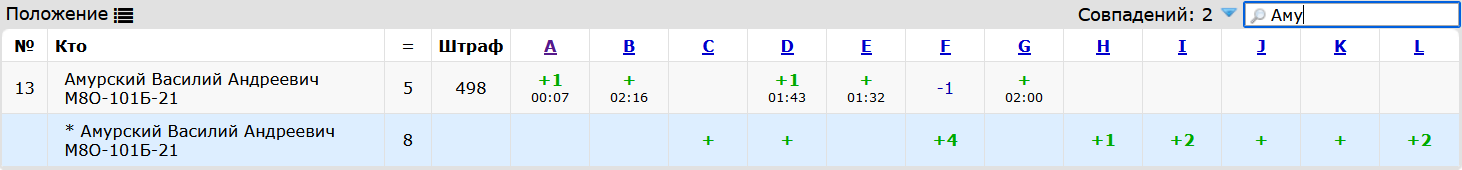
\includegraphics[width=\textwidth]{state6.png}\newline\noindent
\end{center}

\subsubsection*{Выводы}
Задача решена, проблем не возникло.
